Clase: 27/09/2022

\subsection{Homotopía (visión complementaria)}

\begin{definicion}
    Suponga que $\gamma_0:[0,1]\to G$ y $\gamma_1:[0,1]\to G$ son curvas continuas en $G$ que unen los puntos $x_0$ y $x_1\in G\subseteq X$ (espacio topológico). Se dice que $\gamma_0$ es homotópica a $\gamma_1$, denotado $\gamma_0\sim \gamma_1$, si existe una función continua:
    $$H:[0,1]\times[0,1]\to G\ni$$
    \begin{align*}
        H(0,t)&=\gamma_0\\
        H(s,0)&=x_0\\
        H(1,t)&=\gamma_1\\
        H(s,1)&=x_1\\
    \end{align*}

    \begin{figure}[H]
        \centering
        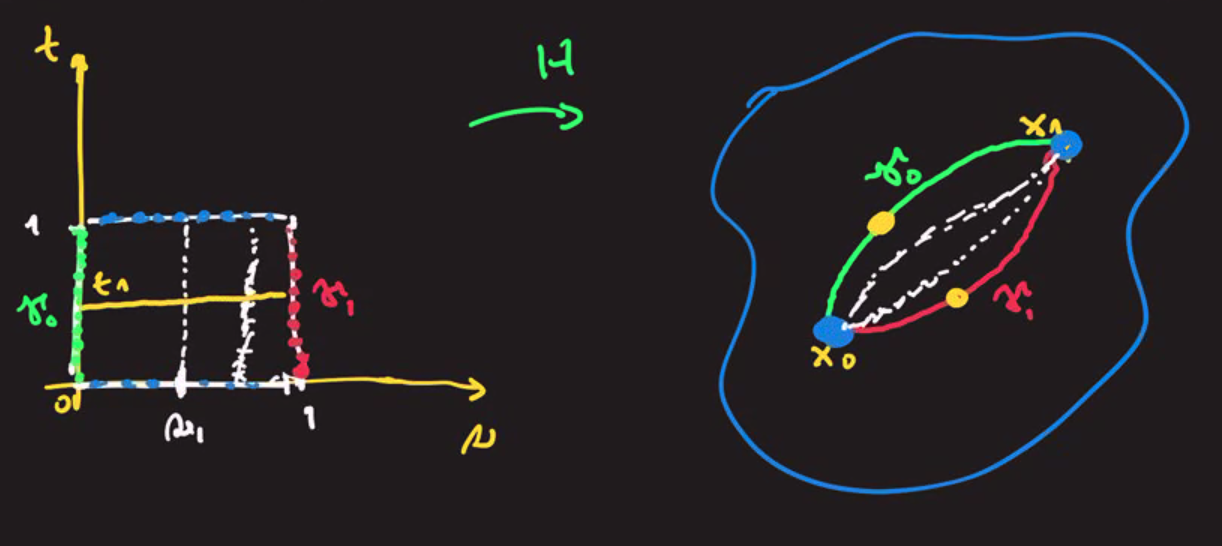
\includegraphics[scale=.3]{imagenes/16.1.png}
    \end{figure}
    
\end{definicion}

\begin{ejemplo}
    Sea $X=\mathbb{R}^2$, entonces el segmento de recta que une $(0,0)$ con $(1,1)$ es homotópico al segmento de parábola que une estos puntos. 
    \begin{figure}[H]
        \centering
        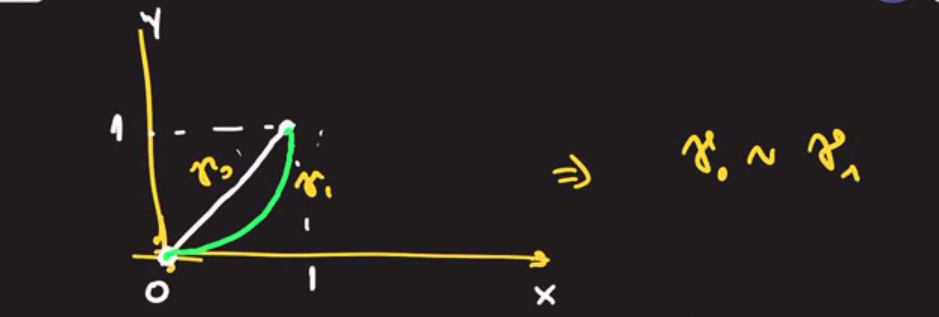
\includegraphics[scale=.3]{imagenes/16.2.png}
    \end{figure}
    Sea $H:[0,1]\times [0,1]\to\mathbb{R}^2\ni$
    $$H(s,t)=(t,t^{s+1})\ni$$
    \begin{align*}
        H(0,t)&=(t,t)=\gamma_0\\
        H(s,0)&=(0,0)=x_0\\
        H(1,t)&=(t,t^2)=\gamma_1\\
        H(s,1)&=(1,1)=x_1\\
    \end{align*}
    Nótese que la homotopía no necesariamente es única. En efecto, sea: 
    \begin{align*}
        H_1(s,t) &= (1-t)\gamma_0(t)+s\gamma_1\\
        H_2(s,t) &= (t,(1-s)t+st^2)
    \end{align*}
\end{ejemplo}


\begin{dem}
    Sean $\gamma_0:[0,1]\to G$ y $\gamma_1:[0,1]\to G$ curvas cerradas simples y continuas en el subconjunto $G$ del espacio topológico $X$. Se dice que $\gamma_0$ es homotópica como curva cerrada a $\gamma_1$ sobre $G$, si existe una función continua 
    $$H:[0,1]\times [0,1]\to G\ni$$
    \begin{align*}
        H(0,t) &= \gamma_0\\
        H(1,t) &= \gamma_1\\
        H(s,0) &= H(s,1)
    \end{align*}
    \begin{figure}[H]
        \centering
        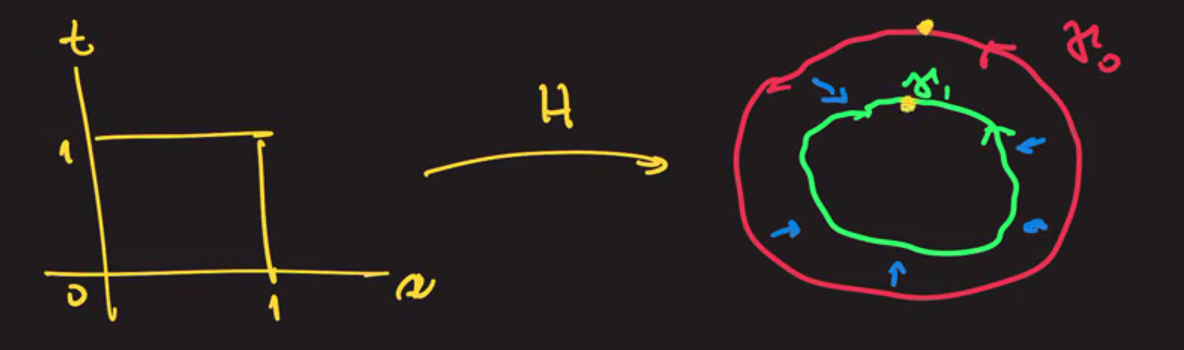
\includegraphics[scale=.3]{imagenes/16.3.png}
    \end{figure}
\end{dem}

\begin{ejemplo}
    El círculo $\gamma_0(t)=(\cos t,\sen t)$ es homotópico a $\gamma_1(t)=(2\cos t,\sen t),t\in [0,2\pi]$ si y solo si 
    \begin{align*}
        \gamma_0(t) &= (\cos 2\pi t,\sin 2\pi t)\\
        \gamma_1(t) &= (2\cos 2\pi t,\sin 2\pi t), t\in [0,1]
    \end{align*}
    Entonces, sea $H:[0,1]^2\to \mathbb{R}^2\ni$ 
    \begin{align*}
        H(s,t)&=\left((1+s)\cos2\pi t, \sin 2\pi t\right),
    \end{align*}
    en donde $H(0,t)=\gamma_0;H(1,t)=\gamma_1,H(s,0)=(1+s,0)=H(s,1)$.
\end{ejemplo}

\begin{nota}
    Sea $\gamma:[0,1]\to X\ni \gamma(t)=x_0$. Nótese que $\gamma$ es una función continua que se le conoce como curva constante (en un punto $x_0\in X$).
\end{nota}

\begin{definicion}
    Un conjunto conexo $A$ del espacio topológico $X$ es simplemente conexo si cada curva cerrada $\gamma$ sobre $A$ es homotópica a un punto en $A$ (i.e. $\gamma\sim x_0$)
\end{definicion}

\subsection{Series}

\begin{prop}
    Sea \begin{itemize}
        \item Si $|r|<1\implies \sum_{n=0}^{\infty}r^n =\frac{1}{1-r}$
        \item Si $|r|\geq 1$, la serie diverge. 
    \end{itemize}
    \begin{dem}
        Sea $S_n=1+r+r^2+\cdots+r^n=\frac{1-r^{n+1}}{1-r}$.
        \begin{enumerate}
            \item Si $|r|<|$ y si $l$. $\implies$ la sucesión $(s_n)$ converge a $1/1-r$. 
            \item Si $|r|>1$ y $n\to\infty\implies r^{n+1}$ diverge a $+\infty\implies (s_n)$ diverge.
            \item Si $r=1\implies \sum_{n=0}^{\infty}1^n =\sum_{n=0}^{\infty}1$. En este caso, $\lim_{n\to\infty}1\neq 0\implies$ la serie diverge. 
        \end{enumerate} 
        

    \end{dem}
    
\end{prop}